\def\sphinxdocclass{report}
\documentclass[a4paper,10pt,english]{sphinxmanual}
\usepackage[utf8]{inputenc}
\DeclareUnicodeCharacter{00A0}{\nobreakspace}
\usepackage{cmap}
\usepackage[T1]{fontenc}
\usepackage{babel}
\usepackage{times}
\usepackage[Sonny]{fncychap}
\usepackage{longtable}
\usepackage{sphinx}
\usepackage{multirow}

%\addto\captionsenglish{\renewcommand{\figurename}{Figure }}
%\addto\captionsenglish{\renewcommand{\tablename}{Table }}
\floatname{literal-block}{Listing }

\usepackage{tabularx}
\usepackage{tabularx}
\usepackage{amsmath}
\usepackage{amsfonts}
\usepackage{amsthm}
\usepackage{amssymb}
\usepackage{booktabs}
\usepackage{tikz}
\usepackage{standalone}
\usepackage{pbox}
\usepackage[procnames]{listings}
\usepackage{courier}
\usepackage{hyperref}

\title{Chondro Documentation}
\date{November 21, 2016}
\release{0.2.3}
\author{Przemyslaw Szufel \\ Bogumi{\l} Kami\'{n}ski \\ Micha{\l} Jakubczyk }
\newcommand{\sphinxlogo}{}
\renewcommand{\releasename}{Release}
\makeindex


\begin{document}
	\pagenumbering{arabic}
	\lstset{language=Python}
	\lstset{escapeinside={(*@}{@*)}}
	\maketitle
	%\phantomsection\label{fun::doc}
	%\index{chondro (module)}\index{bisect() (in module chondro)}

	
\chapter{Decision tree sensitivity analysis with Chondro}

\section{Library overview}
	The goal of this document is to describe the Chobdro library that accompanies our paper titled \emph{``A unified framework for global sensitivity analysis of decision trees''}.

	\emph{Chondro} -- is an analytical engine that implements the decision tree (DT) sensitivity analysis (SA) algorithms described in the above article. All the methods support both for separable and non-separable decision trees. Chondro has been developed with the Python3 and has been tested with Anaconda 2.3.0 running Python3 version 3.4.4. 
	
	The basic Chondro's functionality is described in Table \ref{tab:chondro}. The software can load files stored by the \mbox{SilverDecisions} (available at \url{http://www.silverdecisions.pl}) or uses internal JSON format. A DT is presented as a Python dictionary structure with each node described with a \texttt{type} (choice,decision,final), \texttt{id}, \texttt{value} (pay-off), and a list (\texttt{nodes}) containing child nodes. The probability values \texttt{p} (for separable DTs) or identifiers \texttt{pi} (for non-separable DTs)  are stored in children nodes of a chance node -- full JSON schema specification for DT representation is available at section.  \ref{sec:jsonschema}. For a quick overview please see a sample DT insee Figure \ref{fig:json1}.
	Chondro supports non separable DTs through  injection of probability values as a dictionary. In order to perform stability and perturbation analysis for non-separable decision trees a function that generates probability dictionary on the base of fundamental probabilities should be provided to a respective algorithm. An example of such function has been presented in Listing \ref{lst:codetrans}.
	
	It should be noted that Chondro heavily relies on the Python \texttt{fractions} package for numerical computing and hence enables calculation and comparison of the exact values for P-optimal decisions. In this way we managed to avoid numerical problems when expected values at different nodes are equal.	
	
	\begin{table}
		\begin{tabularx}{\textwidth}{|l|X|X|}
			\hline 
			\textbf{function} & \textbf{description} & \textbf{output}\\ \hline
			\hyperref[index:chondro.load_tree]{\texttt{load\_tree}} & loads a DT from  SilverDecisions or internal \texttt{*.json} file & a Python dictionary holding a decision tree (see Listing \ref{lst:jsonschema} for full DT representation specification)\\ \hline
			\hyperref[index:chondro.save_tree]{\texttt{save\_tree}} & saves a DT to a JSON file & file saved to disk follows format presented in Listing \ref{lst:jsonschema} \\ \hline
			\hyperref[index:chondro.solve_tree]{\texttt{solve\_tree}} & recursively calculates an optimal value for a given separable or non-separable DT & expected value for a tree and P-optimal decisions for every node \\ \hline
			\hyperref[index:chondro.print_tree]{\texttt{print\_tree}} & prints a tree to the standard output & textual representation of a DT -- e.g. see \ref{lst:simpleresults} \\ \hline			
			\hyperref[index:chondro.find_stability]{\texttt{find\_stability}} & finds stability for a separable or non-separable DT & stability coefficient for every optimal decision in a given DT 
			\\ \hline
			\hyperref[index:chondro.find_perturbation_mode]{\pbox{5cm}{
					\texttt{find\_}\texttt{perturbation\_}\\ \texttt{mode}}} & performs a sweep over $\varepsilon$ values in order to find epsilon ranges for $P_{mode}$ perturbation & dictionary of $\varepsilon$ ranges and P-optimal decisions for perturbations
			\\ \hline
			\hyperref[index:chondro.find_perturbation_pessopty]{\pbox{5cm}{
					\texttt{find\_}\texttt{perturbation\_}\\ \texttt{pessopty}}} & performs a sweep over the full grid (non-separable DT) or $\varepsilon$ (separable DT) values and finds epsilon ranges for $P_{\max,\varepsilon}$ and $P_{\min,\varepsilon}$ perturbations & dictionary of $\varepsilon$ ranges and P-optimal decisions for perturbations
			\\ \hline			
		\end{tabularx} 
		\caption{Functionality of the Chondro decision tree sensitivity analysis module}\label{tab:chondro}
	\end{table}	
	
	\begin{figure}
		\centering
		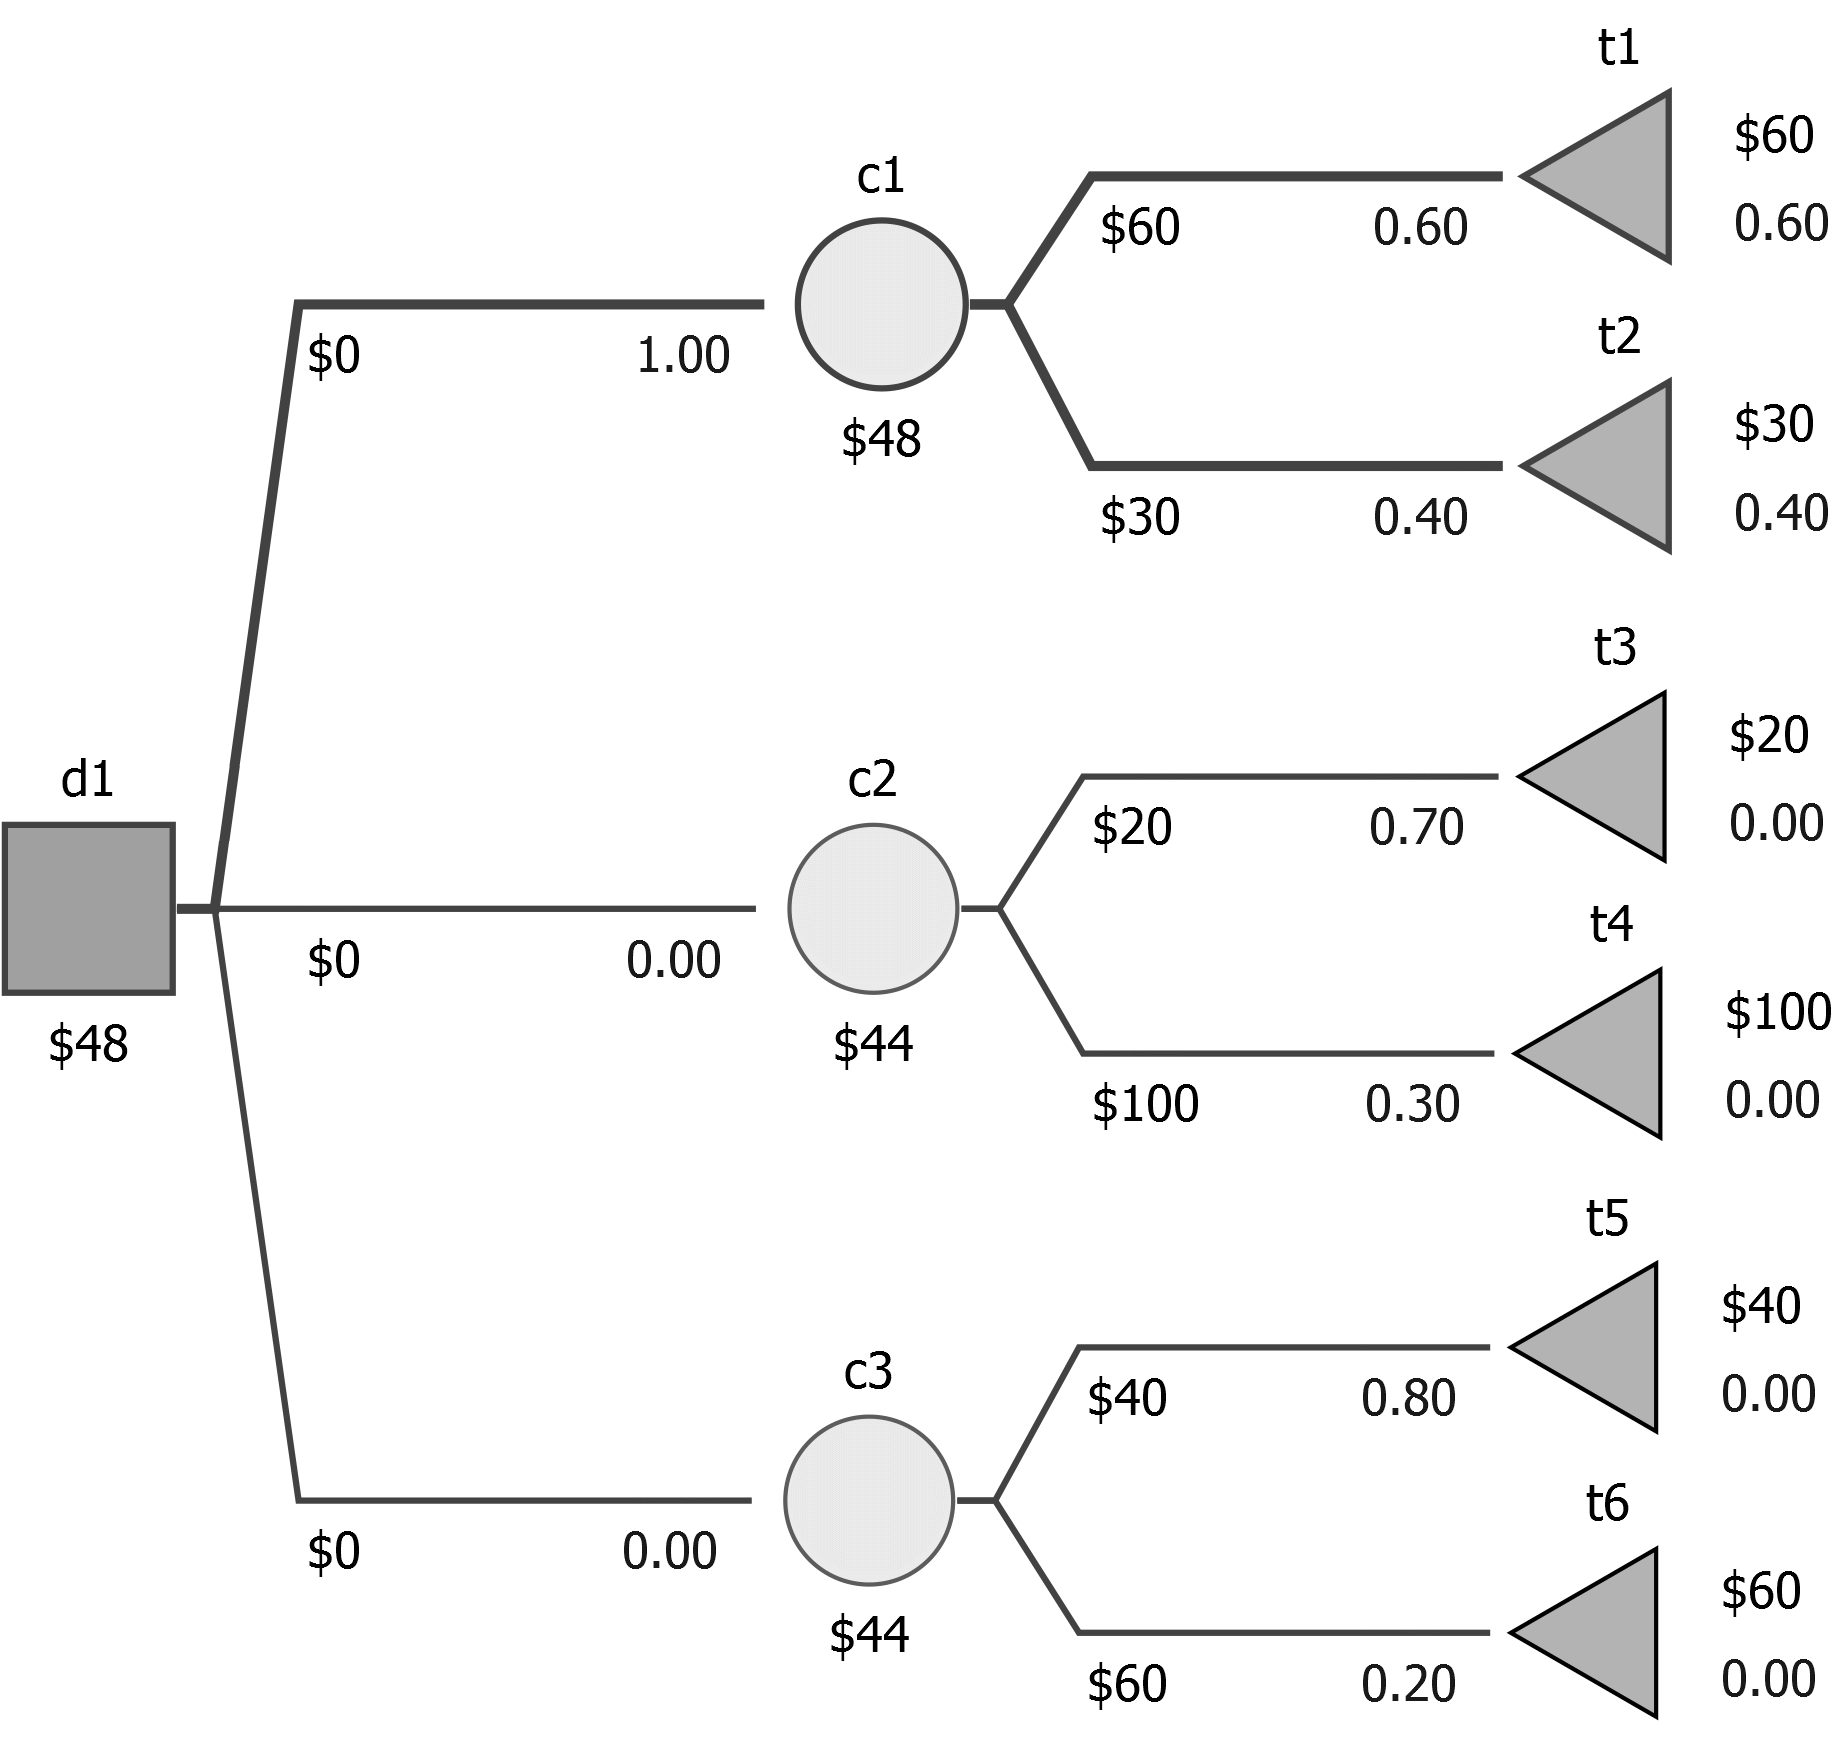
\includegraphics[width=0.65\textwidth]{case1.png}
\begin{lstlisting}[frame=single,label=lst:json1] 
{
  "tree": {
    "type":"decision", "id":"d1",
    "nodes": [
      { 
        "type":"chance","id":"c1",
        "nodes": [
          {"p":"0.6","type":"final","id":"t1","value": "60" },
          {"p":"0.4","type":"final","id":"t2","value": "30" }        
        ]             
      },
      { 
        "type":"chance","id":"c2",
        "nodes": [
          {"p":"0.7","type":"final","id":"t3","value": "20" },
          {"p":"0.3","type":"final","id":"t4","value": "100" }        
        ]             
      },
      { 
        "type":"chance","id":"c3",
        "nodes": [
          {"p":"0.8","type":"final","id":"t5","value": "40" },
          {"p":"0.2","type":"final","id":"t6","value": "60" }             
        ]
      }     
    ]
  }
}



\end{lstlisting}
		\caption{A separable decision tree and a corresponding JSON representation. The probability and payoff values are given as string rather than number values in order to enable a proper conversion with the \texttt{fractions} module. The full JSON schema decision tree specification see Listing \ref{lst:jsonschema}.}
		\label{fig:json1}
\end{figure}


	\begin{figure}
		\centering
		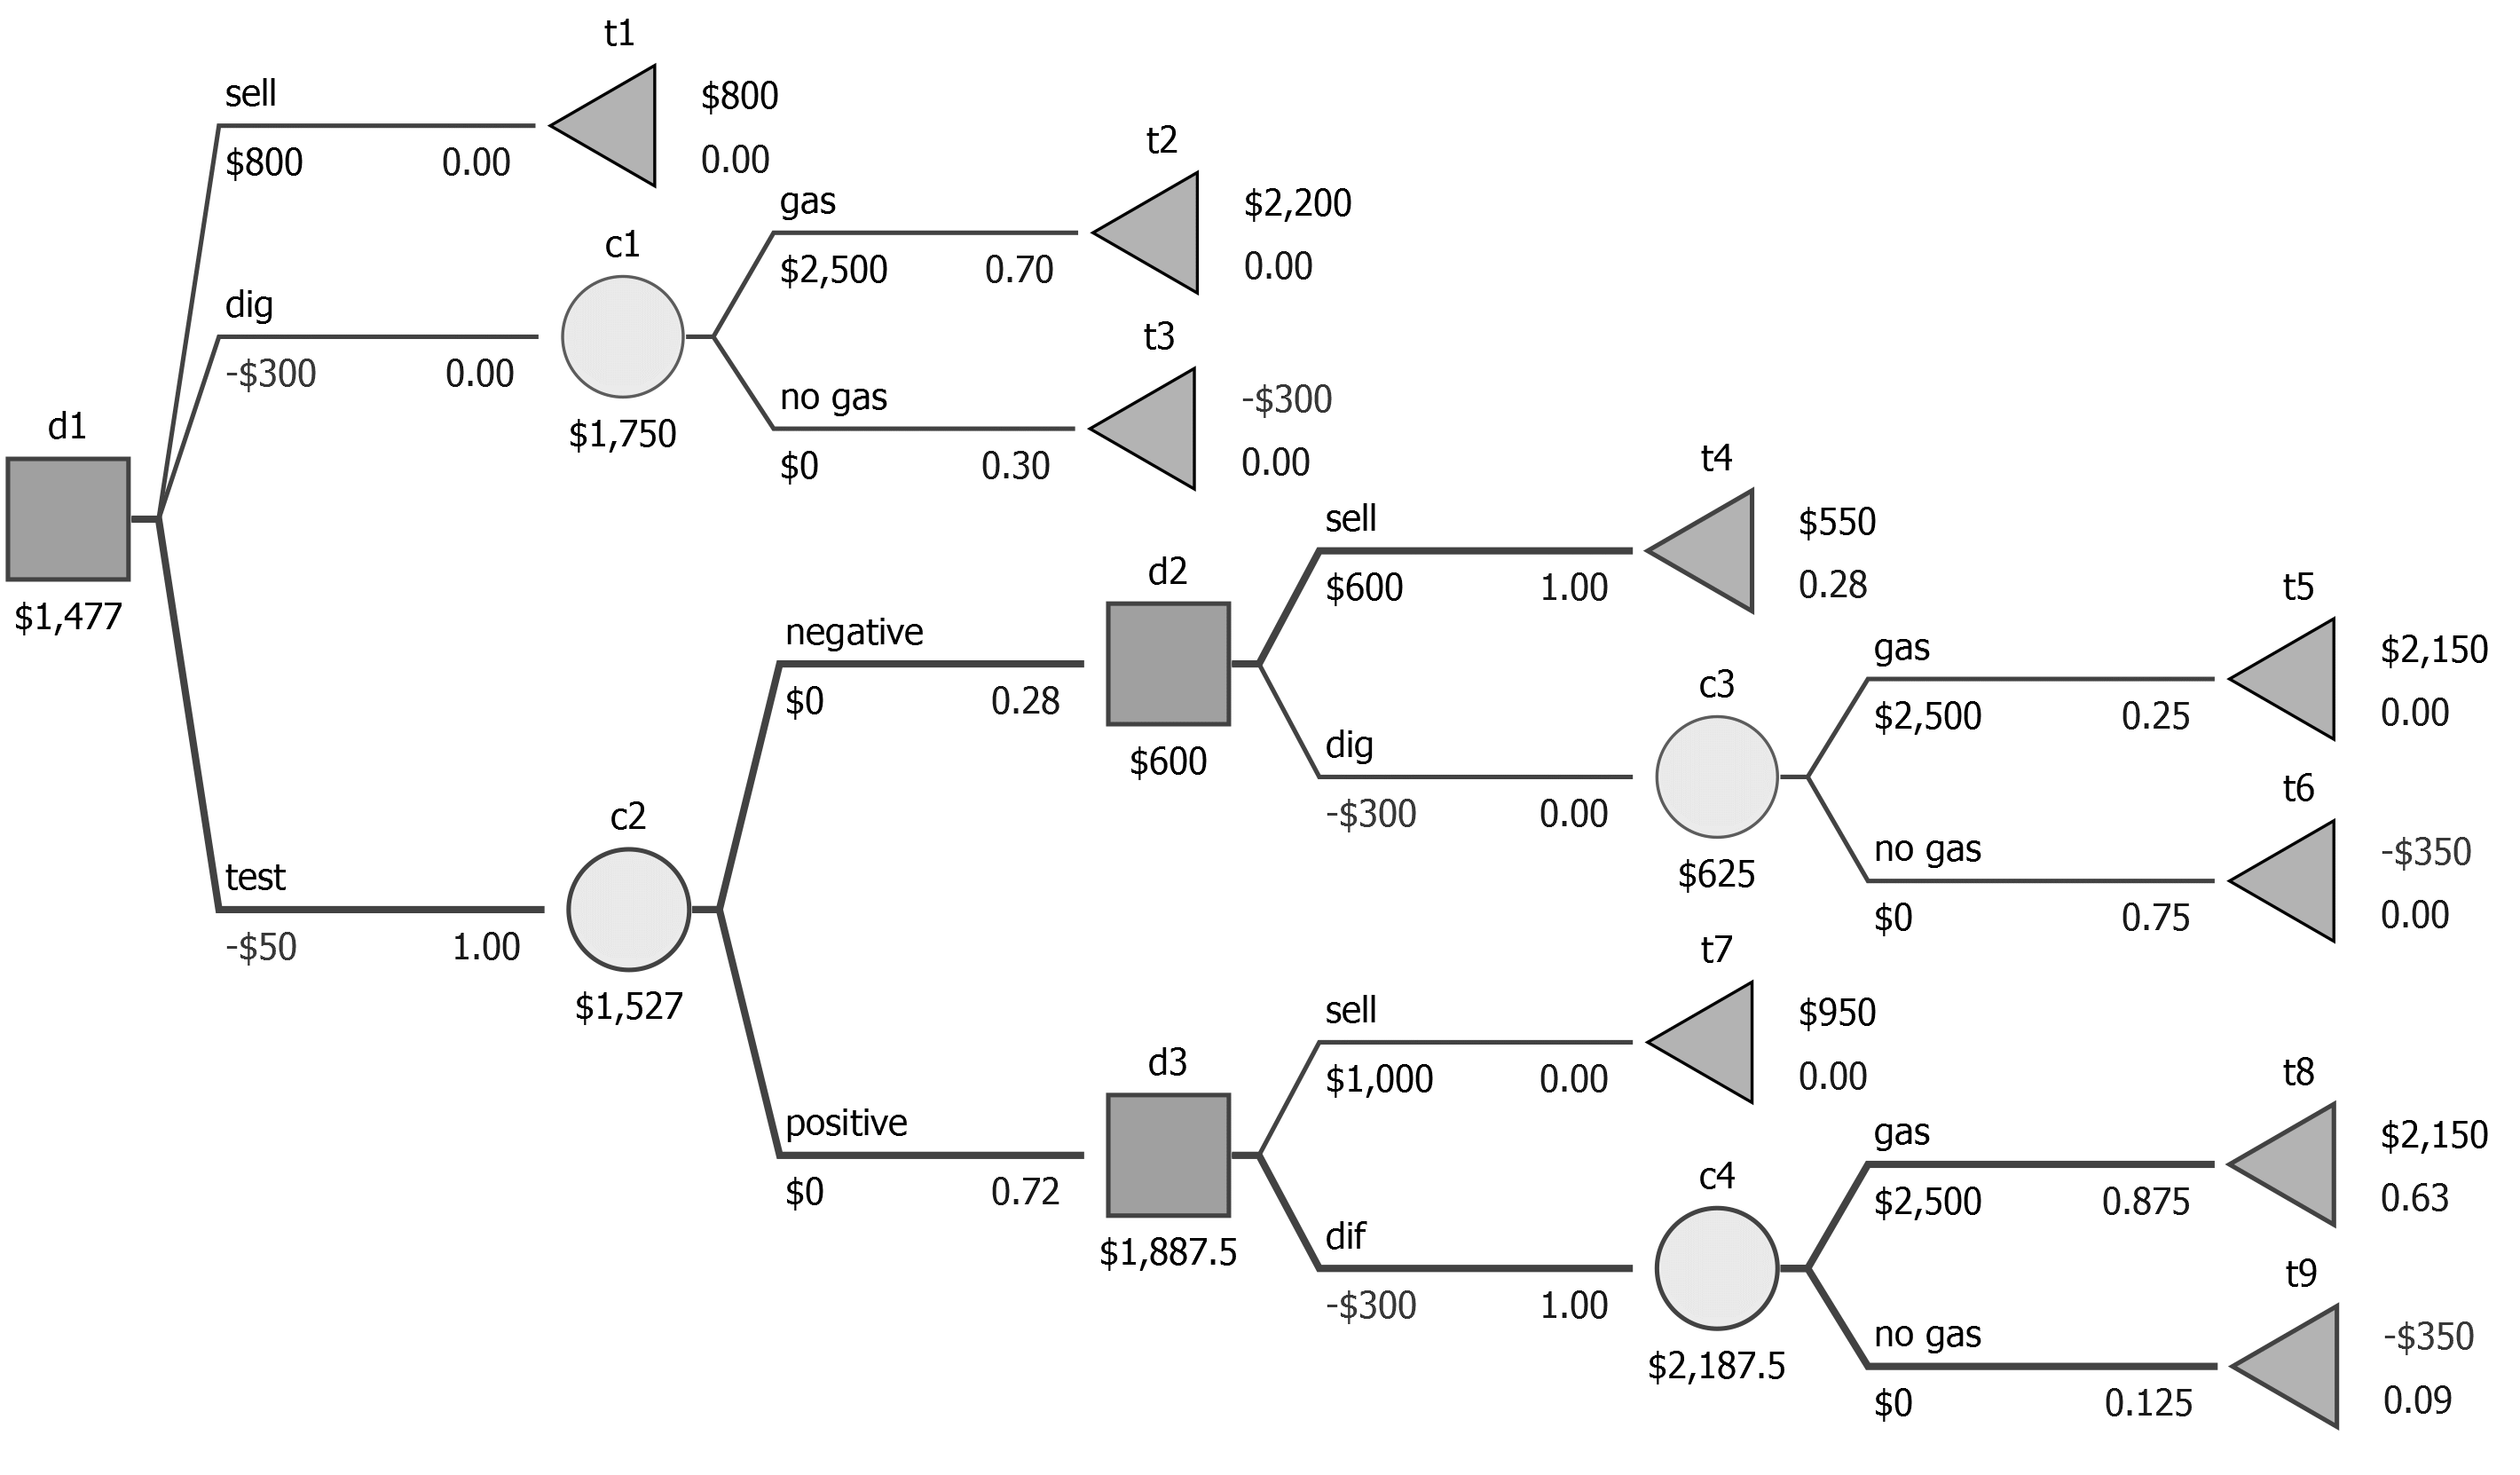
\includegraphics[width=0.85\textwidth]{gas.png}
\begin{lstlisting}[frame=single,label=lst:json2] 
{
    "tree": {
        "type": "decision", "id": "d1",
        "nodes": [
            {
                "type": "final","label":"sell","id": "t1","value": "800"
            }, 
            {
                "type": "chance","label":"dig","id": "c1","value": "-300",
                "nodes": [
                    {
                        "pi": "gas", "label":"gas",
                        "type": "final", "id": "t2", "value": "2500"
                    }, 
                    {
                        "pi": "no_gas", "label":"no_gas",
                        "type": "final", "id": "t3", "value": "0"
                    }
                ] 
            }, 
            {
                "type": "chance","label":"test","id": "c2","value": "-50",
                "nodes": [
                    {
                        "pi": "neg._test", "label":"negative",
                        "type": "decision", "id": "d2",
                        "nodes": [
                            {
                                "type": "final", 
                                "label":"sell",
                                "id": "t4", 
                                "value": "600"
                            }, 
(...)
\end{lstlisting}
		\caption{A non-separable decision tree and a part of the corresponding JSON representation.}
		\label{fig:json2}
\end{figure}


	
	\section{Quick start - sensitivity analysis of separable trees}
	A typical example session with  Chondro might consist of the following steps:
	\begin{enumerate}
		\item create a JSON representation of a DT (either by saving a DT from SilverDecisions or manually creating a JSON file)		
		\item Use the \hyperref[index:chondro.load_tree]{\texttt{load\_tree}} function to load a DT to memory
		\item Use the \hyperref[index:chondro.solve_tree]{\texttt{solve\_tree}} function to calculate optimal decision for the DT. The function supports non-separable trees by accepting a probability dictionary.
		\item perform the sensitivity analysis
		\begin{itemize}
			\item use \hyperref[index:chondro.find_stability]{\texttt{find\_stability}} to calculate the stability 
			\item use \hyperref[index:chondro.find_perturbation_mode]{\texttt{find\_perturbation\_mode}} to calculate $P_{mode,\varepsilon}$
								
			\item use \hyperref[index:chondro.find_perturbation_pessopty]{
					\texttt{find\_perturbation\_pessopty}} to calculate $P_{\min,\varepsilon}$ and $P_{\max,\varepsilon}$
		\end{itemize}

	\end{enumerate}
	
	Listing \ref{lst:codesimple} presents a sample code to solve the decision tree. We first start by loading the module (line \ref{py:import}). Next a JSON file is loaded with the \hyperref[index:chondro.load_tree]{\texttt{load\_tree}}  function. It should be noted that this function supports JSON files in both internal dictionary format as well as files that can be exported from SilverDecisions software (available at \url{http://www.silverdecisions.pl}). The function \hyperref[index:chondro.solve_tree]{\texttt{solve\_tree}} (line \ref{py:solve}) returns a tuple where the first element is the expected value of DT and the second dictionary of optimal decisions. 
	
	It should be noted that in Chondro a decision tree is represented as a python dictionary - a direct representation of the JSON file presented in the Figure \ref{fig:json1}. We assume that each node in a tree can be identified by a path represented as a Python tuple of indices. The root node is represented by \texttt{()} (an empty tuple) the first node (\texttt{c1} in Listing \ref{lst:simpleresults}) is represented by \texttt{(0,)} (one element tuple) while the node \texttt{t3}  could be presented as \texttt{(1,0)}. Node paths are used to for represent $P$-optimal decisions. Further in the text the tuple of node indices representing a path in the graph will be called \texttt{node\_path\_tuple}.  It should be noted that all sensitivity analysis methods (\hyperref[index:chondro.find_stability]{\texttt{find\_stability}},
	\hyperref[index:chondro.find_perturbation_mode]{\texttt{find\_perturbation\_mode}} and  \hyperref[index:chondro.find_perturbation_pessopty]{\texttt{find\_perturbation\_pessopty}}) provide a \texttt{use\_labels} parameter. If it is set to \texttt{True} (the default value) Chondro uses  \texttt{label} attribute (see section \ref{sec:jsonschema}) of decision tree nodes rather than indices to represent paths in the tree. For example consider a DT in Figure \ref{fig:json2}. The $P$-optimal decision can be presented a tuple of two \texttt{node\_path\_tuple}s either as \texttt{((2, 0, 0), (2, 1, 1))} or  \texttt{(("test", "negative", "sell"), ("test", "positive", "dig"))}. The $P$-optimal decision consists of two elements because the test performed at c2 node can have two results - can be either positive or negative. Further in the text a tuple of \texttt{node\_path\_tuple}s will be called \emph{\texttt{decision\_path\_tuple}}.
	
	The function \hyperref[index:chondro.solve_tree]{\texttt{solve\_tree}} returns the optimal decision paths in the form of a following dictionary:	
	\begin{equation*}
	 \texttt{\{ node\_path\_tuple : [\textit{list of $P$-optimal node indices}] \}}
	\end{equation*}
	It should be noted that the function \hyperref[index:chondro.solve_tree]{\texttt{solve\_tree}} changes the state of the \texttt{tree} object -- now additionally it stores the data on optimal solution. The function \hyperref[index:chondro.print_tree]{\texttt{print\_tree}} enables printing a human-readable textual representation of a DT to the console (line \ref{py:print}). A sample textual tree representation can be found in Listing \ref{lst:simpleresults}.  
	
	Once a decision tree is loaded and solved a sensitivity analysis (SA) can be performed. The first step is calculating the stability value and $P_{mode,\varepsilon}$. The function \hyperref[index:chondro.find_stability]{\texttt{find\_stability}} (line \ref{py:fs}) returns results in the form of the following dictionary of $P$-optimal decisions:
	\begin{equation*}
	\texttt{\{ decision\_path\_tuple : stability\_epsilon \} }
	\end{equation*}
	
	In the next step, the  $P_{mode,\varepsilon}$ perturbations is calculated (line \ref{py:pm}). The output of the \hyperref[index:chondro.find_perturbation_mode]{\texttt{find\_perturbation\_mode}} function is the following:
	\begin{equation*}
	\texttt{\{ (e1,e2) : [\textit{list of} decision\_path\_tuple\textit{s}] \}}
	\end{equation*}
	where \texttt{e1} and \texttt{e2} represent some range of $\varepsilon$ values where the set of $P$-optimal decisions does not change (please node that a decision tree can have more than one $P$-optimal decision and hence a list is here used).
	
	Finally, $P_{\min,\varepsilon}$ and $P_{\max,\varepsilon}$ are calculated with the function \hyperref[index:chondro.find_perturbation_pessopty]{\texttt{find\_perturbation\_pessopty}} (line \ref{py:pp}). The results will be returned in the following format:
	\begin{equation*}
	\begin{split}	
		\texttt{\{ }
		\texttt{"max\_min" : \{ (e1,e2) : [\textit{list of} decision\_path\_tuple\textit{s}] \},}\\
		\texttt{"max\_max" : \{ (e1,e2) : [\textit{list of} decision\_path\_tuple\textit{s}] \}}
		\texttt{ \}}				  
	\end{split}				
	\end{equation*}	
	Both elements of the above dictionary (\texttt{"max\_min"} and \texttt{"max\_max"}) are analogous to the output of the \hyperref[index:chondro.find_perturbation_mode]{\texttt{find\_perturbation\_mode}} function. The value of \texttt{"max\_min"} represents $P_{\min,\varepsilon}$ perturbation sensitivity while the value of \texttt{"max\_max"} represents $P_{\max,\varepsilon}$ perturbation sensitivity.


	It should be noted that for separable tree analysis Chondro supports the $s\colon\mathcal{C}\rightarrow[0,1]$ function representing whether a given chance node should be subject to sensitivity analysis. Simply add the \texttt{s} property to any chance node in a separable tree. The default value is $\texttt{s}=1$ i.e. all chance nodes in a separable tree will be considered in sensitivity analysis of a DT.

	\noindent\begin{minipage}{\linewidth}
		\begin{lstlisting}[frame=single,caption=Source code for separable probability,label=lst:codesimple,numbers=left] 
(*@\label{py:import}@*)from chondro import *

file_name = "example_separable_Fig5.json"
tree = load_tree(file_name)
(*@\label{py:solve}@*)ev,dec=solve_tree(tree)
print ("DT has been solved, the expected value is ev: "+str(ev)+ \
       " reachable decisions: "+str(get_reachable(dec)))

(*@\label{py:print}@*)print_tree(tree)

(*@\label{py:fs}@*)stabi = find_stability(tree,precision=Fraction("1/10000") )
print ("DT stability", stabi)

(*@\label{py:pm}@*)ress = find_perturbation_mode(tree,precision=Fraction("1/1000"))
print("DT perturbation mode",ress)

(*@\label{py:pp}@*)ress = find_perturbation_pessopty(tree,precision=Fraction("1/1000"))
for key in ress.keys():
	print ("P_"+key, ress[key])		
\end{lstlisting}
		
\end{minipage}		
		
\noindent\begin{minipage}{\linewidth}
\begin{lstlisting}[frame=single, caption={Textual representation of decision tree from Figure \ref{fig:json1} in Chondro. For each chance node the probabilities \texttt{p} are given and the expected values \texttt{ev} have been calculated. The asterix (*) represents the optimal decision(s).  It should be noted that Chondro uses \texttt{fractions} package and hence the results can be calculated utilizing full precision.} ,label=lst:simpleresults]		
d1:decision
  *c1:chance (ev=48)
    t1:p=3/5 final [60]
    t2:p=2/5 final [30]
   c2:chance (ev=44)
    t3:p=7/10 final [20]
    t4:p=3/10 final [100]
   c3:chance (ev=44)
    t5:p=4/5 final [40]
    t6:p=1/5 final [60]
\end{lstlisting}		
\end{minipage}	

	

	
\section{Sensitivity analysis of non-separable trees}

The Chondro library is capable of processing both separable and non separable trees. Due to much larger computational complexity of non-separable the library has different internal implementation of stability and perturbation algorithms for both tree types. A sample non-separable decision tree has been presented in Figure \ref{fig:json2}.

The support for non-separable trees is achieved by providing to the function \hyperref[index:chondro.solve_tree]{\texttt{solve\_tree}} an additional parameter \texttt{derived\_probs\_dict} that contains a dictionary of key-probability values that can be injected into \texttt{pi} fields in a decision tree. Hence, there are two differences in processing non-separable DTs compared to separable ones:
\begin{itemize}
	\item probabilities in the decision tree are represented as keys rather than values and use \texttt{pi} fields instead of \texttt{p} fields. 
	\item in order to perform sensitivity analysis a function needs to be provided that transforms fundamental probabilities into dictionary of key-value pairs that can be injected by Chondro into \texttt{pi} fields in a DT
\end{itemize}


Calculating stability and perturbation requires performing a sweep over a set of fundamental probabilities and providing a function transferring those probabilities into a key-probability dictionary. Hence, the methods  \hyperref[index:chondro.find_stability]{\texttt{find\_stability}},  \hyperref[index:chondro.find_perturbation_pessopty]{
		\texttt{find\_perturbation\_pessopty}} and \hyperref[index:chondro.find_perturbation_mode]{
		\texttt{find\_perturbation\_mode}} require providing two additional parameters:
\begin{itemize}
	\item \emph{derived\_probs\_lambda} - a function that calculates derived probabilities     on the  base of fundamental ones. The function should return a dictionary where keys are corresponding to \texttt{pi} values in a decision tree.
	
	\item \emph{fundamental\_probs} - a list of initial vales of fundamental probabilities
\end{itemize}
	
An example function that calculates probabilities on the base of fundamental ones has been presented in (e.g. see Listing \ref{lst:codetrans}. 

The initial values for fundamental probabilities is represented as a list of events where each event is described by a list of outcome probabilities. Moreover, if there are $n$ possible outcomes of an event the probabilities of $n-1$ should be only passed - the last $n$-th probability will be automatically calculated.
For example suppose that we consider two fundamental probabilities result of throwing a coin and a result of throwing a four-sided dice. In that case the fundamental probabilities in Chondro will be presented as: \texttt{[[0.5],[0.25,0.25,0.25]]}. 

In Listing \ref{lst:codetrans} an example processing of a non-separable decision tree has been presented. Firstly, fundamental probabilities values need to be defined (line \ref{py:sep_fund_probs}). Those values can be used to calculate a $P$-optimal decision (line \ref{py:sep_solve}). In the line \ref{py:sep_s} we defined $s$ values representing whether a particular event (for which fundamental probabilities have been given) should be a subject of sensitivity analysis. 
Finally, we perform the stability analysis - in our computations we limit the maximum considered value of $\varepsilon$ to $1$. 
	
\noindent\begin{minipage}{\linewidth}
	\begin{lstlisting}[frame=single,caption=Source code for function transforming separable probabilities (\texttt{probs}) into non-separable probabilities at nodes of the tree presented in Figure \ref{fig:json2},label=lst:codetrans] 
def tree_derived_probs_lambda(probs): 
	p=dict()
	p["gas"] = probs[0][0]
	sensitivity = probs[1][0]
	specifity = probs[2][0]
	p["no_gas"] = 1-p["gas"]
	p["pos._test"]=sensitivity*p["gas"]+  \
	(1-specifity)*p["no_gas"]
	p["neg._test"]=1-p["pos._test"]
	p["gas|pos._test"]=sensitivity*p["gas"]/p["pos._test"]
	p["no_gas|pos._test"]=1-p["gas|pos._test"]
	p["gas|neg._test"]=(1-sensitivity)*p["gas"]/  \
	p["neg._test"]
	p["no_gas|neg._test"]=1-p["gas|neg._test"]
	return p
	\end{lstlisting}
\end{minipage}

\noindent\begin{minipage}{\linewidth}
	\begin{lstlisting}[frame=single,caption={Calculating sensitivity analysis for a separable decision tree with Chondro. We have assumed that the function tree\_derived\_probs\_lambda has been defined as presented in Listing \ref{lst:codetrans}.} ,label=lst:separable,numbers=left] 
from chondro import *

tree = load_tree("exaple_non_separable_fig7.json")
(*@\label{py:sep_fund_probs}@*)fund_probs = [[Fraction("7/10")],[Fraction("9/10")],[Fraction("7/10")]]
(*@\label{py:sep_solve}@*)solve_tree(tree,tree_derived_probs_lambda(fund_probs))
print_tree(tree)
(*@\label{py:sep_s}@*)s = [1,0.1,0.1]
stabi = find_stability(tree,tree_derived_probs_lambda, \
          fund_probs,precision=Fraction("1/100"),s=s,max_epsilon=1) )
print ("stability", stabi)
ress = find_perturbation_mode(tree,tree_derived_probs_lambda,\
         fund_probs,precision=Fraction("1/100"),s=s,max_epsilon=1))
print("mode perturbation",ress)
ress = find_perturbation_pessopty(tree,tree_derived_probs_lambda,\
         fund_probs,precision=Fraction("1/100"),s=s,max_epsilon=1) )
for key in ress.keys():
    print ("P "+key, ress[key])
	\end{lstlisting}
\end{minipage}





\chapter{Reference manual}	
\section{List of available functions}
\begin{fulllineitems}
	\phantomsection\label{index:chondro.bisect}\pysiglinewithargsret{\code{chondro.}\bfcode{bisect}}{\emph{fun}, \emph{a}, \emph{b}, \emph{precision=1e-06}, \emph{divide=2.0}}{}
	Implements bisection with a given precision.
	
	\emph{fun} - a boolean function
	
	\emph{a} - start value
	
	\emph{b} - end value
	
	\emph{precision} - precision parameter
	
	\emph{divide} - division parameter
	
	examples:
	
	bisect(lambda x: x*x-5 \textgreater{} 0, 0.0,5.0)
	
	bisect(lambda x: x*x-5 \textgreater{} 0, Fraction(0),Fraction(5),divide=Fraction(2))
	
\end{fulllineitems}

\index{bisect\_change() (in module chondro)}

\begin{fulllineitems}
	\phantomsection\label{index:chondro.bisect_change}\pysiglinewithargsret{\code{chondro.}\bfcode{bisect\_change}}{\emph{fun}, \emph{start\_value}, \emph{a}, \emph{b}, \emph{precision=1e-06}}{}
	Implements bisection with a given precision - searching for a change 
	in function value.
	
	\emph{fun} - a boolean function
	
	\emph{start\_value} - a starting value of the function
	
	\emph{a} - start value
	
	\emph{b} - end value
	
	\emph{precision} - precision parameter
	
	returns x where the change was observed and the new function value
	
\end{fulllineitems}

\index{find\_gamma\_probs() (in module chondro)}

\begin{fulllineitems}
	\phantomsection\label{index:chondro.find_gamma_probs}\pysiglinewithargsret{\code{chondro.}\bfcode{find\_gamma\_probs}}{\emph{probs}, \emph{e}}{}
	Finds a gamma value for the most probable values.
	
	\emph{probs} - a list of probabilities
	
	\emph{e} - epsilon
	
	examples:
	
	find\_gamma\_probs({[}Fraction(``1/4''),Fraction(``3/8''),Fraction(``3/8''){]},    Fraction(0.249999))
	
	find\_gamma\_probs({[}Fraction(``1/4''),Fraction(``3/8''),Fraction(``3/8''){]},    Fraction(0.25))
	
	find\_gamma\_probs({[}Fraction(``1/4''),Fraction(``3/8''),Fraction(``3/8''){]},0.1)
	
\end{fulllineitems}

\index{find\_perturbation\_mode() (in module chondro)}

\begin{fulllineitems}
	\phantomsection\label{index:chondro.find_perturbation_mode}\pysiglinewithargsret{\code{chondro.}\bfcode{find\_perturbation\_mode}}{\emph{tree}, \emph{derived\_probs\_lambda=None}, \emph{grouped\_fundamental\_probs=None}, \emph{precision=Fraction(1}, \emph{100)}, \emph{max\_epsilon=None}, \emph{s=None}, \emph{use\_labels=True}}{}
	Finds peturbation stability for mode-perturbation type
	The grid contains the original probabilities as well as the corner cases 
	(probabilities equal to zero and one).
	
	\emph{tree} - a decision tree represented as a dictionary
	
	\emph{derived\_probs\_lambda} - a function that calculates derived probabilities
	on the base of fundamental ones
	
	\emph{grouped\_fundamental\_probs} - a list of groups of fundamental probabilities
	
	\emph{precision} - step value for the gamma parameter sweep
	
	\emph{max\_epsilon} - maksimum epsilon value considered in the computation
	
	\emph{s} - sensitivity list for fundamental probabilities
	
	\emph{use\_labels} - decisions will be presented as labels rather than indices
	
	Output format:	
	\begin{equation*}
		\texttt{\{ (e1,e2) : [\textit{list of} decision\_path\_tuple\textit{s}] \}}
	\end{equation*}
	where \texttt{e1} and \texttt{e2} represent some range of $\varepsilon$ values where the set of $P_{mode,\varepsilon}$ does not change (please node that a decision tree can have more than one $P$-optimal decision and hence a list is here used).
	
\end{fulllineitems}

\index{find\_perturbation\_pessopty() (in module chondro)}

\begin{fulllineitems}
	\phantomsection\label{index:chondro.find_perturbation_pessopty}\pysiglinewithargsret{\code{chondro.}\bfcode{find\_perturbation\_pessopty}}{\emph{tree}, \emph{derived\_probs\_lambda=None}, \emph{grouped\_fundamental\_probs=None}, \emph{precision=Fraction(1}, \emph{10)}, \emph{max\_epsilon=None}, \emph{s=None}, \emph{use\_labels=True}}{}
	Performs a full grid sweep search in order to find $P_{\min,\varepsilon}$ and $P_{\max,\varepsilon}$ values.
	The grid contains the original probabilities as well as the corner cases 
	(probabilities equal to zero and one).
	If only epsilon stability is selected the search stops after finding the
	first set of fundamental probabilities that changes the decision.
	
	\emph{tree} - a decision tree represented as a dictionary
	
	\emph{derived\_probs\_lambda} - a function that calculates derived probabilities     on the base of fundamental ones
	
	\emph{fundamental\_probs} - a list of groups of fundamental probabilities
	
	\emph{step} - step value for the parameter sweep
	
	\emph{max\_epsilon} - maksimum epsilon value for parameter sweep generation
	
	\emph{s} - the s parameter for fundamental probabilities
	
	\emph{use\_labels} - decisions will be presented as labels rather than indices
	
	Output format:	
	\begin{equation*}
		\begin{split}	
			\texttt{\{ }
			\texttt{"max\_min" : \{ (e1,e2) : [\textit{list of} decision\_path\_tuple\textit{s}] \},}\\
			\texttt{"max\_max" : \{ (e1,e2) : [\textit{list of} decision\_path\_tuple\textit{s}] \}}
			\texttt{ \}}				  
		\end{split}				
		\end{equation*}	
		 The value of \texttt{"max\_min"} represents $P_{\min,\varepsilon}$ perturbation sensitivity while the value of \texttt{"max\_max"} represents $P_{\max,\varepsilon}$ perturbation sensitivity. \texttt{e1} and \texttt{e2} represent some range of $\varepsilon$ values where the set of $P$-optimal decisions does not change (please node that a decision tree can have more than one $P$-optimal decision and hence a list is here used).
	
\end{fulllineitems}

\index{find\_stability() (in module chondro)}

\begin{fulllineitems}
	\phantomsection\label{index:chondro.find_stability}\pysiglinewithargsret{\code{chondro.}\bfcode{find\_stability}}{\emph{tree}, \emph{derived\_probs\_lambda=None}, \emph{grouped\_fundamental\_probs=None}, \emph{precision=Fraction(1}, \emph{10)}, \emph{max\_epsilon=None}, \emph{s=None}, \emph{use\_labels=True}}{}
	Finds the stability coefficient for every optimal decision
	in a given separable or nonseparable tree.
	
	\emph{tree} - a decision tree represented as a dictionary
	
	\emph{derived\_probs\_lambda} - a function that calculates derived probabilities     on the  base of fundamental ones
	
	\emph{fundamental\_probs} - a list of groups of fundamental probabilities
	
	\emph{precision} - precision (for separable) or sweep step     (for non separable trees)
	
	\emph{max\_epsilon} - maximum value of an epsilon in the sweep
	
	\emph{s} - sensitivity list for fundamental probabilities
	
	\emph{use\_labels} - decisions will be presented as labels rather than indices
		
	Returns results in the form of the following dictionary of $P$-optimal decisions:		
	\begin{equation*}
		\texttt{\{ decision\_path\_tuple : stability\_epsilon \} }
		\end{equation*}
	
\end{fulllineitems}

\index{full\_sweep() (in module chondro)}

\begin{fulllineitems}
	\phantomsection\label{index:chondro.full_sweep}\pysiglinewithargsret{\code{chondro.}\bfcode{full\_sweep}}{\emph{grouped\_probs}, \emph{step=Fraction(1}, \emph{5)}, \emph{max\_epsilon=None}, \emph{s=None}}{}
	Generates a parameter sweep for a given set of grouped probabilities
	The corner probabilities 0 and 1 are included in the sweep if they are 
	in the max\_epsilon range.
	
	The sum of probabilities in any group does not exceed 1.
	
	\emph{grouped\_probs} - a list of probabilities groups {[}{[}p1, p2{]},{[}p3{]},{[}p4,p5{]}{]}
	
	\emph{step} - step value used to generate the parameter sweep
	
	\emph{max\_epsilon} - maximum value of an epsilon in the sweep
	
\end{fulllineitems}

\index{get\_decision\_name() (in module chondro)}

\begin{fulllineitems}
	\phantomsection\label{index:chondro.get_decision_name}\pysiglinewithargsret{\code{chondro.}\bfcode{get\_decision\_name}}{\emph{tree}, \emph{path\_tuple}}{}
	Transforms a given \emph{path\_tuple} to a tuple of node labels from 
	a given decision \emph{tree}
	
\end{fulllineitems}

\index{get\_reachable() (in module chondro)}

\begin{fulllineitems}
	\phantomsection\label{index:chondro.get_reachable}\pysiglinewithargsret{\code{chondro.}\bfcode{get\_reachable}}{\emph{dec}}{}
	For a given decision strategy dictionary creates a copy 
	with removed optimal decisions that are not reachable.
	
	\emph{dec} - decision dictionary
	
	example:
	
	get\_reachable(\{():{[}0,1{]},(1,):{[}2,3{]},(2,):{[}1,2{]},(2,2):{[}0{]}\})      will return  \{(): {[}0, 1{]}, (1,): {[}2, 3{]}\} because the nodes (2,) and (2,2)     cannot be reached - at the root node the only optimal decisions are 0 and 1
	
\end{fulllineitems}

\index{go\_fractions() (in module chondro)}

\begin{fulllineitems}
	\phantomsection\label{index:chondro.go_fractions}\pysiglinewithargsret{\code{chondro.}\bfcode{go\_fractions}}{\emph{node}}{}
	Recursively enables Fractions for a dictionary decision tree.
	The parameter types of `p' and `value' fields are changed fractions
	
	\emph{node} - tree or subtree
	
\end{fulllineitems}

\index{load\_tree() (in module chondro)}

\begin{fulllineitems}
	\phantomsection\label{index:chondro.load_tree}\pysiglinewithargsret{\code{chondro.}\bfcode{load\_tree}}{\emph{file\_name}, \emph{use\_fractions=True}}{}
	Loads a decision tree defintion from a give file.
	The file can be either a plain dict saved to JSON or a SilverDecisions 
	file. If a SilverDecisions file has several trees only the first decision tree in a file is read.
	
	\emph{file\_name} - a name of the file
	
	\emph{use\_fractions} - should ``fractions'' module be used for computational     accurancy
	
\end{fulllineitems}

\index{node\_branching() (in module chondro)}

\begin{fulllineitems}
	\phantomsection\label{index:chondro.node_branching}\pysiglinewithargsret{\code{chondro.}\bfcode{node\_branching}}{\emph{node}, \emph{\_\_branching=()}}{}
	Creates a set of all possible decisions for a given decision tree.
	
	\emph{node} - root node of a decision tree
	
\end{fulllineitems}

\index{perturb() (in module chondro)}

\begin{fulllineitems}
	\phantomsection\label{index:chondro.perturb}\pysiglinewithargsret{\code{chondro.}\bfcode{perturb}}{\emph{probs}, \emph{v}, \emph{epsilon}, \emph{maximize}}{}
	Calculates a peturbation for a given parameter set
	
	\emph{probs} - list initial probabilities
	
	\emph{v} - payoff values
	
	\emph{epsilon} - max perturbation
	
	\emph{maximize} - maximize (True) or minimize payoff (False)
	
\end{fulllineitems}

\index{print\_tree() (in module chondro)}

\begin{fulllineitems}
	\phantomsection\label{index:chondro.print_tree}\pysiglinewithargsret{\code{chondro.}\bfcode{print\_tree}}{\emph{node}, \emph{\_\_level=0}}{}
	Recursively prints a decision tree subtree.
	
	\emph{node} - tree root or sub-node
	
	\emph{\_\_level} - internal parameter of the function - level of the tree
	
\end{fulllineitems}

\index{save\_tree() (in module chondro)}

\begin{fulllineitems}
	\phantomsection\label{index:chondro.save_tree}\pysiglinewithargsret{\code{chondro.}\bfcode{save\_tree}}{\emph{tree}, \emph{file\_name}, \emph{overwrite=False}}{}
	Saves the tree definition to a file.
	
	\emph{tree} - a dictionary representation of a decision tree
	
	\emph{file\_name} - a name of the file
	
	\emph{overwrite} - should the file be overwritten if it exists
	
\end{fulllineitems}

\index{solve\_tree() (in module chondro)}

\begin{fulllineitems}
	\phantomsection\label{index:chondro.solve_tree}\pysiglinewithargsret{\code{chondro.}\bfcode{solve\_tree}}{\emph{node}, \emph{derived\_probs\_dict=None}, \emph{node\_stability\_type=None}, \emph{decision=None}, \emph{\_\_branching=()}, \emph{\_\_best\_path=None}}{}
	Recursive method to find an optimal value for a decision tree.
	
	\emph{node} - tree or sub-tree to be calculated
	
	\emph{derived\_probs\_dict} - dictionary of probabilities for non-separable trees
	(if present a node will use those probability values instead of `p')
	
	\emph{node\_stability\_type} - a lambda (probs,evs,best\_path,s) to recalculate     probabilities at chance nodes
	
	\emph{decision} - decision dictionary to calculate ev of a tree for     a particular decision
	
	\emph{\_\_branching} - internal method parameter - current position in the tree
	
	\emph{\_\_best\_path} - internal method parameter - best paths in the tree
	
	The function returns a tuple: \texttt{(expected\_value, optimal\_decisions\_dictionary)}. The optimal decision dictionary is presented as the following: 
	\begin{equation*}
		 \texttt{\{ node\_path\_tuple : [\textit{list of $P$-optimal node indices}] \}}
		\end{equation*}
	
	WARNING! The function has the following side effects on the tree parameter:
	\begin{itemize}
		\item expected values of chance nodes will be saved in the `ev' field
		
		\item children of a decision node will store a `best' boolean field with \texttt{True} value indicating $P$-optimal decisions
		
	\end{itemize}
	
\end{fulllineitems}

\index{tree\_branching\_to\_tuple() (in module chondro)}

\begin{fulllineitems}
	\phantomsection\label{index:chondro.tree_branching_to_tuple}\pysiglinewithargsret{\code{chondro.}\bfcode{tree\_branching\_to\_tuple}}{\emph{tree\_branching}, \emph{use\_names\_tree=None}}{}
	Converts a full decision dictionary to a tuple of tuples.
	
	\emph{tree\_branching} - list of dictionaries generated with tree\_sweep
	
	\emph{use\_names\_tree} - use labels from decision tree     rather than indices to represent nodes
	
	example
	tree\_branching\_to\_tuple(\{():{[}1{]},(1,): {[}2{]},(1,2):{[}3,4{]}\})
	yields
	(((1, 2, 3),), ((1, 2, 4),))
	
\end{fulllineitems}

\index{tree\_decision\_paths\_to\_tuple() (in module chondro)}

\begin{fulllineitems}
	\phantomsection\label{index:chondro.tree_decision_paths_to_tuple}\pysiglinewithargsret{\code{chondro.}\bfcode{tree\_decision\_paths\_to\_tuple}}{\emph{tree\_sweep\_decision}}{}
	Converts a decision dictionary to a list decision.
	
	example:
	
	tree\_decision\_paths\_to\_tuple(\{():{[}1{]},(1,): {[}2{]},(1,2):{[}3{]}\})
	
	returns ((1, 2, 3),)
	
\end{fulllineitems}

\index{tree\_sweep() (in module chondro)}

\begin{fulllineitems}
	\phantomsection\label{index:chondro.tree_sweep}\pysiglinewithargsret{\code{chondro.}\bfcode{tree\_sweep}}{\emph{decision\_dictionary}}{}
	Transforms a \emph{decision\_dictionary} to list of dictionaries,
	with single decisions in each node.
	
	example:
	
	tree\_sweep(\{(1,):{[}1,2{]}\})
	
	returns {[}\{(1,): {[}1{]}\}, \{(1,): {[}2{]}\}{]}
	
\end{fulllineitems}


\section{Decision tree format specification}\label{sec:jsonschema}

Listing \ref{lst:jsonschema} presents a specification JSON schema a decision tree. It should be noted that \texttt{p} and \texttt{value} fields accept both \texttt{number} and \texttt{string} values. The textual values enable entering rational numbers in \texttt{fractions} module format (e.g. \texttt{1/7}) and thus avoiding loss of precision. It should be noted that when using \texttt{string} to represent numbers in a DT the function  \hyperref[index:chondro.load_tree]{\texttt{load\_tree}} requires using the default value (\texttt{True}) of the parameter \texttt{use\_fractions}.

The \texttt{p} value in chance node children is used to represent possibilities as real numbers while the \texttt{pi} value is used to represent a field in a dictionary that will be passed to the \hyperref[index:chondro.solve_tree]{\texttt{solve\_tree}}  function.

The fields \texttt{ev} and \texttt{best} are added to the tree when the \hyperref[index:chondro.solve_tree]{\texttt{solve\_tree}} is called in order to indicate expected values on the chance nodes and best paths in a DT. It should be noted that the function \hyperref[index:chondro.save_tree]{\texttt{save\_tree}} does not store values of those fields.

\begin{lstlisting}[frame=single,label=lst:jsonschema,caption={JSON schema for the decision tree representation. }] 
{
  "$schema": "http://json-schema.org/draft-04/schema#",
  "definitions": {
    "node": {
      "type": "object",
      "properties": {
        "value": { "type": ["string","number"] },
        "id": { "type": "string" },
        "label": { "type": "string" }
      }
    },
    "probabilities": {
      "type": "object",
       "properties": {
          "p": { "type":  ["string","number"] },
          "pi": { "type":  "string"}
       },
       "oneOf" : [{"required" : ["p"]},{"required" : ["pi"]}]
    },
    "best": {
      "type": "object",
       "properties": {"best": { "type":  "boolean" }}      
    },
    "node-decision": {
      "allOf": [
        {"$ref": "#/definitions/node" },
        { "properties" : {
          "type":{"type":"string","enum": ["decision"]},
          "nodes": {
            "type": "array",
            "items": { "oneOf": [
	           {"allOf": [
	             { "$ref": "#/definitions/node-decision" },
	             { "$ref": "#/definitions/best" }
	           ]},
	           {"allOf": [
	             { "$ref": "#/definitions/node-chance" },
	             { "$ref": "#/definitions/best" }
	           ]},
	           {"allOf": [
	             { "$ref": "#/definitions/node-final" },
	             { "$ref": "#/definitions/best" }
	           ]}
	         ]
            }
          }
        }}
      ],
      "required": ["type","nodes"]
    },
    "node-final": {
      "allOf": [
        {"$ref": "#/definitions/node" },
        { "properties" : {
          "type":{"type":"string","enum": ["final"]}          
        }}
      ],
      "required": ["type","value"]
    },
    "node-chance": {
      "allOf": [
        {"$ref": "#/definitions/node" },
        { "properties" : {
          "type":{"type":"string","enum": ["chance"]},
          "s":{"type":"number"},          
          "ev":  {"type":"number"},
          "nodes": {
            "type": "array",
            "items": { "oneOf": [
              {"allOf": [
                { "$ref": "#/definitions/node-decision" },
                { "$ref": "#/definitions/probabilities" }
              ]},
              {"allOf": [
                { "$ref": "#/definitions/node-chance" },
                { "$ref": "#/definitions/probabilities" }
              ]},
              {"allOf": [
                { "$ref": "#/definitions/node-final" },
                { "$ref": "#/definitions/probabilities" }
              ]}
            ]
            }
          }
        }}
        ],
        "required": ["type","nodes"]
    }     
  },
  
  "type": "object",
  "properties": {
    "tree": { "oneOf": [
              { "$ref": "#/definitions/node-decision" }, 
              { "$ref": "#/definitions/node-chance" }, 
              { "$ref": "#/definitions/node-final" } 
              ]
            }
  },
  "required": ["tree"]
}
\end{lstlisting}
	
\end{document}
